%%%%%%%%%%%%%%%%%%%%%%%%%%%%%%%%%%%%%%%%%
% fphw Assignment
% LaTeX Template
% Version 1.0 (27/04/2019)
%
% This template originates from:
% https://www.LaTeXTemplates.com
%
% Authors:
% Class by Felipe Portales-Oliva (f.portales.oliva@gmail.com) with template 
% content and modifications by Vel (vel@LaTeXTemplates.com)
%
% Template (this file) License:
% CC BY-NC-SA 3.0 (http://creativecommons.org/licenses/by-nc-sa/3.0/)
%
%%%%%%%%%%%%%%%%%%%%%%%%%%%%%%%%%%%%%%%%%

%----------------------------------------------------------------------------------------
%	PACKAGES AND OTHER DOCUMENT CONFIGURATIONS
%----------------------------------------------------------------------------------------

\documentclass[
	12pt, % Default font size, values between 10pt-12pt are allowed
	%letterpaper, % Uncomment for US letter paper size
	%spanish, % Uncomment for Spanish
]{fphw}

% Template-specific packages
\usepackage[utf8]{inputenc} % Required for inputting international characters
\usepackage[T1]{fontenc} % Output font encoding for international characters
\usepackage{mathpazo} % Use the Palatino font
\usepackage[dvipsnames]{xcolor}
\usepackage{graphicx} % Required for including images
\usepackage{amsmath}
\usepackage{booktabs} % Required for better horizontal rules in tables
\usepackage{listings} % Required for insertion of code
\usepackage{enumerate} % To modify the enumerate environment
\usepackage{ragged2e}
\usepackage{cancel}
\usepackage{MnSymbol,bbding,pifont}
\usepackage{lscape}
\usepackage{array}
\usepackage{float,graphicx}
\usepackage{hyperref}
\newcolumntype{M}{>{$}c<{$}}
%----------------------------------------------------------------------------------------
%	ASSIGNMENT INFORMATION
%----------------------------------------------------------------------------------------

\title{Assignment \#4} % Assignment title

\author{Luis Alberto Ballado Aradias} % Student name

\date{\today} % Due date

\institute{Centro de Investigación y de Estudios Avanzados del IPN \\ Unidad Tamaulipas} % Institute or school name

\class{Tecnologías Computacionales (Sep - Dec 2022)} % Course or class name

\professor{Dr. Edwin Aldana Bobadilla} % Professor or teacher in charge of the assignment

%----------------------------------------------------------------------------------------

\begin{document}

\maketitle % Output the assignment title, created automatically using the information in the custom commands above

%----------------------------------------------------------------------------------------
%	ASSIGNMENT CONTENT
%----------------------------------------------------------------------------------------
{\color{teal}
\dotfill
Undecidable Problems
\dotfill}

In computability theory, an \textbf{undecidable problem} is a type of computational problem that requires a yes/no answer, but where there cannot possibly be any computer program that always gives the correct answer; that is, any possible program would sometimes give the wrong answer or run forever without giving any answer.\\
More formally, an \textbf{undecidable problem} is a problem whose language is \textbf{not a recursive set}\\

Now talking about Decidability in terms of a Turing machine, a problem is said to be a \textbf{Decidable problem} if there exists a corresponding Turing machine which halts on every input with an answer \textbf{yes or no}. It is also important to know that these problems are termed as \textbf{Turing Decidable} since Turing machine always halts on every input, accepting or rejecting it.\\

Undecidable problems can be related to different topics, such as \textbf{logic}, \textbf{abstract}, \textbf{machines} or \textbf{topology}. Since there are \textbf{uncountably} many undecidable problems, any list, even one of infinite length, is necessarily incomplete.\\

There are some problems that a computer can never solve, even the world's most powerful computer with infinite time: the undecidable problems.\\

Computer scientists and mathematicians have discovered many more undecidable problems. Quite a few of those, once simplified, look like another case of the halting problem. Generally, all the undecidable problems revolve around the difficulty of determining properties about the input and output of programs. It's helpful to realize when we're dealing with an undecidable problem. We can then accept that our program can't correctly answer yes or no on all inputs, and come up with a different approach.

\begin{itemize}
\item The Halting Problem
\item Post Correspondence Problem
\item Wang tiles  
\item Diophantine equations
\end{itemize}

\newpage
\section*{{\color{BlueViolet}The Halting Problem}}

Alan Turing proved the existence of undecidable problems in 1936 by finding an example, the now famous \textbf{halting problem}. Based on its code and an input, will a particular program ever finish running?\\

For example, consider this program that counts down:\\

\begin{verbatim}
num = 10
REPEAT UNTIL (num = 0){
  DISPLAY(num)
  num = num - 1
}
\end{verbatim}

That program will halt, since num eventually becomes 0.\\
Compare that to this program that counts up:

\begin{verbatim}
num = 10
REPEAT UNTIL (num = 0){
  DISPLAY(num)
  num = num + 1
}
\end{verbatim}

It counts up forever, since num will never equal 0.\\

Algorithms do exist that can correctly predict that the first program halts and the second program never does. These are simple programs which donot change based on different inputs. \textbf{However, no algorithm exists that can analyze any program's code and determine whether it halts or not.} In order to prove that such an algorithm cannnot possibly exist, Turing used a \textbf{proof of contradiction}.\\

We start by imagining that an algorithm does exist that can determine a program's haltability. Then we propose a program called HaltChecker that takes two inputs, a program's code and an input for that program. It then uses that hypothetical haltability algorithm to return either \textbf{halts} or \textbf{never halts}.\\

This flow chart visualizes HaltChecker:

\begin{figure}[H]
  \centering
  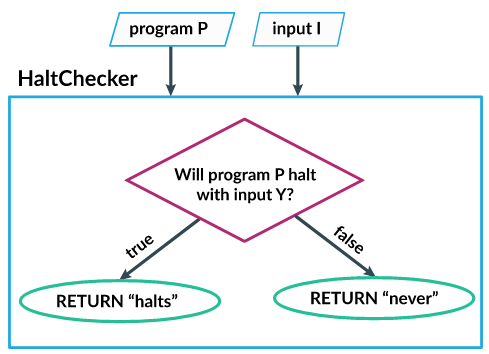
\includegraphics[scale=0.4]{images/halting.png}
\end{figure}

\newpage
\section*{{\color{Apricot}Post Correspondence Problem}}

This is a popular \textbf{undecidable problem} that was introduced by Emil Leon Post back in 1946. It is simpler than Halting Problem. In this problem we have N number of Dominos. The aim is to arrange tiles in such order that string made by Numerators is same as string made by Denominators. In simple words, lets assume we have two list both containing N words, aim is to fing out concatenation of these words in some sequence such that both list yield same result. Let's try understanding this by taking two list A and B.

\begin{verbatim}
A=[aa, bb, abb] and B=[aab, ba, b]
\end{verbatim}

Now for sequence 1,2,1,3 first list will yield aabbaaabb and second list will yield same string aabbaaabb. So the solution to this PCP becomes 1,2,1,3. Post Correspondence Problems can be represented in two ways.

\begin{itemize}
\item Domino's Form
  \begin{figure}[H]
  \centering
  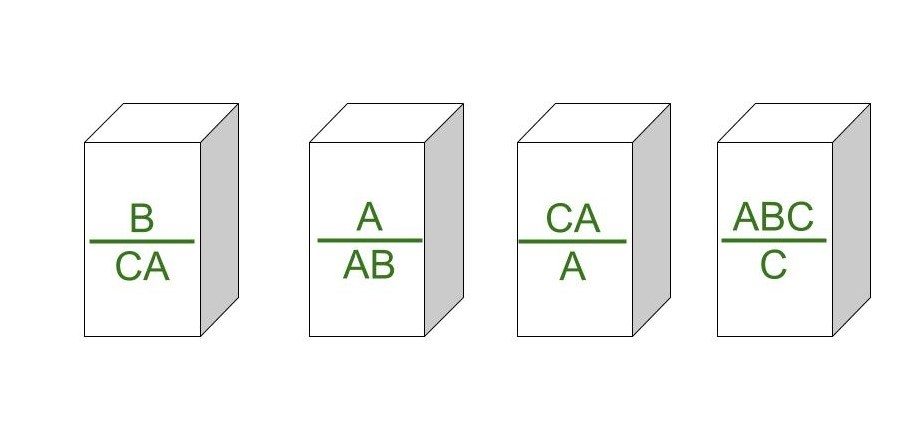
\includegraphics[scale=0.4]{images/dominos.jpg}
\end{figure}
\item Table Form
  \begin{figure}[H]
  \centering
  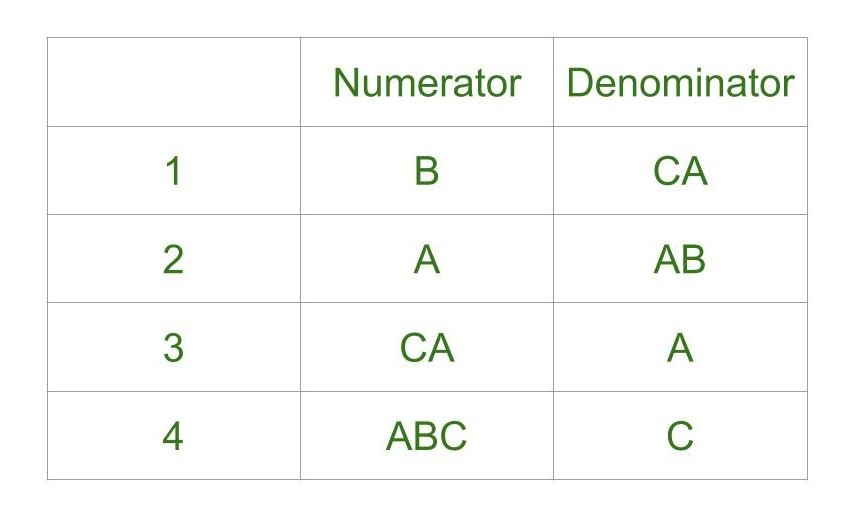
\includegraphics[scale=0.4]{images/table.jpg}
\end{figure}
\end{itemize}

We can try unlimited combinations like one above but none of combination will lead us to solution, thus this problem does not have solution.\\
There is no particular algorithm that determines whether any Post Correspondence System has solution or not.

\section*{{\color{Cerulean}Wang tiles}}

\begin{figure}[H]
  \centering
  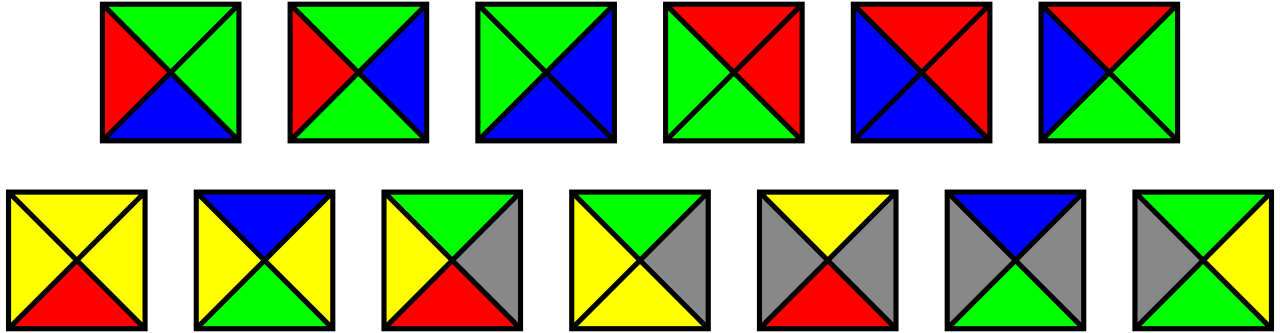
\includegraphics[scale=0.3]{images/wang.png}
\end{figure}

A Wang tile (or simply tile) is a unit square tile with colored edges and a Wang tile set is a finite set of Wang tiles. A tiling by Wang tiles is a mapping which assigns a unique tile from the given tile set for each location of the plane. A tiling is said to be valid if the colors of neighboring tiles match. The tiling problem of Wang tiles (also known as the domino problem) is the decision problem of determining whether a given finite tile set admits at least one valid tiling. It was shown by Berger that the tiling problem is undecidable.\\

Wang tiles have been used previously, for example, to prove undecidability of injectivity and surjectivity of two-dimensional cellular automata and nilpotency of one-dimensional cellular automata. The definition of determinism for tile sets was originally motivated by the theory of one-dimensional cellular automata.\\

A tile set can be considered as a one-dimensional cellular automaton, if the tile set contains all the possible color pairs at one corner and the tile set is deterministic by the same corner. The tiles can be seen as states of the cells and the diagonal rows of tiles as configurations of the cellular automaton. Therefore, the rule, which determines whether neighboring tiles match, can in this case be considered as the local rule of a cellular automaton.\\

It has been shown that the tiling problem is undecidable with tile sets that are deterministic by at least one corner. From this it follows that nilpotency of one-dimensional cellular automata is undecidable. Undecidability of nilpotency follows from the fact that a tiling error can be used to create a spreading quiescent state in the local rule and then every diagonal row of tiles leads to a quiescent configuration if, and only if, there exists no valid tiling.\\

If a Wang tile set is deterministic by two opposite corners, then the tile set can be seen as a subset of the state set of a reversible one-dimensional cellular automaton. In fact, knowing that the tiling problem is undecidable for 2-way deterministic tile sets (i.e. tile sets that are deterministic by two opposite corners), one can prove certain properties of reversible one-dimensional cellular automata to be undecidable. From the tiling problem itself it follows that it is undecidable if for any initial configuration some cell always enters a \textbf{forbidden} state representing a tiling error. It is also undecidable if for any initial configuration every cell eventually enters a forbidden state. Using a reduction from the tiling problem of 2-way (or 4-way) deterministic tile sets, it can also be shown that a weaker form of expansivity, left expansivity (or right expansivity), is undecidable.

\newpage
\section*{{\color{RoyalPurple}Diophantine equations}}

Does the equation $x^{3}+y^{3}+z^{3}=29$ have a solution in integers?, YES: (3,1,1), for instance. How about $x^{3}+y^{3}+z^{3}=30?$, again YES, although this was not know until 1999: the smallest solution is (-283059965, -2218888517, 222042293). And how about $x^{3}+y^{3}+z^{3}=33$? This is an unsolved problem.\\
Of course, number theory does not end with the study of cubic equations in three variables one might ask also about $x^{1729}y^{1093}z^{196884}-163xyzt^{262537412638648300}=561$.\\

D. Hilbert, in the list of 23 problems he published after a famous lecture in 1900, asked his audience to find a method that would answer all such questions. More precisely, Hilbert’s tenth problem (hereafter denoted H10) asks for an algorithm that takes as input a multivariable polynomial $f (x1, . . . , xn)$ with integer coefficients and outputs YES or NO according to whether there exist integers $a_{1},a_{2},..,a_{n}$ such that $f(a_{1},....,a_{n})=0$.\\

In 1970, Yu. Matiyasevich, building on earlier work of M. Davis, H. Putnam, and J. Robinson, showed that no such algorithm exists.\\

Diophantine analysis\\

Typical questions
\begin{enumerate}
\item Are there any solutions?
\item Are there any solutions beyond some that are easily found by inspection?
\item Are there finitely or infinitely many solutions?
\item Can all solutions be found in theory?
\item Can one in practice compute a full list of solutions?
\end{enumerate}



references:\\
\url{https://www.geeksforgeeks.org/post-correspondence-problem/}\\
\url{https://www.cs.odu.edu/~zeil/cs390/latest/Public/undecidable/index.html}\\
\url{https://en.wikipedia.org/wiki/Undecidable_problem}\\
\url{https://en.wikipedia.org/wiki/Diophantine_equation}\\

\end{document}
